\chapter{Regularizacija}

Pri vpeljavi linearne regresije v prejšnjem poglavju je bil cilj
gradnja modela, ki se čimbolj prilega učni množici. Pa je to res pravi
kriterij za določanje parametrov modela? Bo model, ki se najbolje
prileže učni množici res tisti, ki bo dobro napovedoval nove primere?
V tem poglavju pokažemo, da temu ni tako, nakažemo, kakšna bi bila
lahko rešitev problema in potem tudi povemo, da je ta žal odvisna od
parametra, ki ga moramo nekako oceniti iz podatkov. S tem smo sklenili
začarani krog (in morda nismo rešili prav dosti), a odprli skrinjico
problemov, ki je tipična za strojno učenje in znanost v podatkih.

\section{Polinomska regresija}

Na sliki~\ref{fig:poly-linear} so prikazani podatki, kjer linearni model očitno ni pravi in je odvisnost med atributom in razredom nelinearna. Linearni model z enim samim atributom, oziroma tako imenovani univariatni linearni model, očitno ne bo kos našemu problemu. 

\begin{figure}[htbp]
\begin{center}
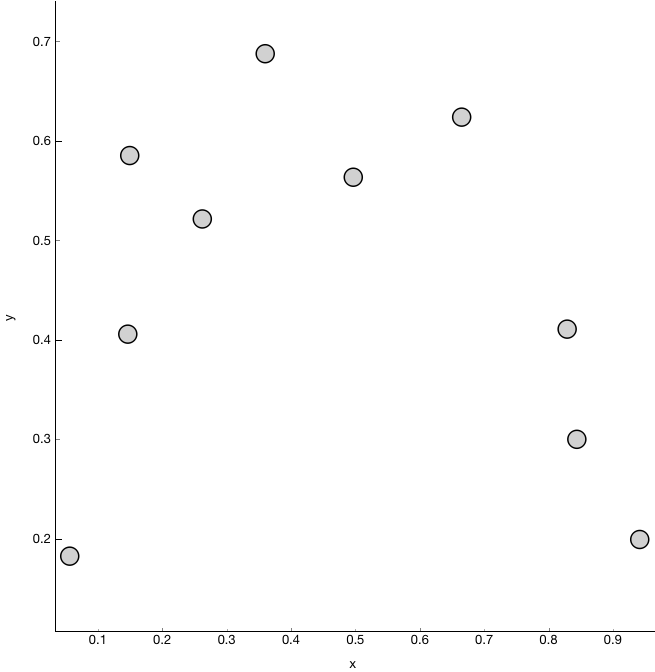
\includegraphics[width=0.45\textwidth]{slike/poly-linear.png}
\caption{Linearni model $y=\theta_0 + \theta_1 x$ se ne ujema dobro s podatki, saj je napaka velika, odvisnost med atributom $x$ in razredom $y$ pa očitno ni linearna.}
\label{fig:poly-linear}
\end{center}
\end{figure}

Model z eno samo spremenljivko zapišemo kot $y=\theta_0 + \theta_1 x$. Kaj pa, če podatke spremenimo tako, da število atributov povečamo. S stolpci, ki so potence našega osnovnega atributa. Torej, namesto, da vhodni podatki vsebujejo samo stolpec z atributom $x$, dodamo še stolpce potenc te spremenljivke, torej na primer stolpce z vrednostmi $x^2$ in $x^3$. Za trenutek uvedimo nova imena spremenljivk, oziroma nova imena atributov, in poimenujmo $a=x$, $b=x^2$ in $c=x^3$. S takimi spremenljivkami lahko zapišemo novi linearni model $y=\theta_0 + \theta_1 a + \theta_2 b + \theta_3 c$. S takimi modeli smo tudi že imeli opravka (v prejšnjem poglavju), zato nam niso novi. Še vedno gre za linearni model: torej model, kjer so $a$, $b$ in $c$ neke številke (vrednosti atributov za posamezni primer), ki so pomnožene s parametri modela $\theta_0\ldots\theta_3$, katerih vrednost iščemo.

Sedaj pa preoblikujmo naš model tako, da spet vstavimo potence atributa $x$. Tokrat se zavedajmo, da potenčni izrazi označujejo vrednosti atributov, torej nekih konstant iz naše tabele podatkov. Prav zato je model še vedno linearen:

$$ y=\theta_0 + \theta_1 x + \theta_2 x^2 + \theta_3 x^3 $$

Pravimo, da smo prostor atributov razširili s potenčnimi vrednostmi. Ker bomo nad tem prostorom gradili linearni regresijski model, temu postopku razširitve prostora atributov in gradnje linearnega modela pravimo polinomska regresija. In rezultat? Na sliki~\ref{fig:poly-linear-fit} je prikazan rezultat pri polinomski razširitvi stopnje 2 (uporabili smo atributa $x$ in $x^2$) ter stopnje štiri (uporaba atributov $x$, $x^2$, $x^3$ in $x^4$).

\begin{figure}[htbp]
\begin{center}
  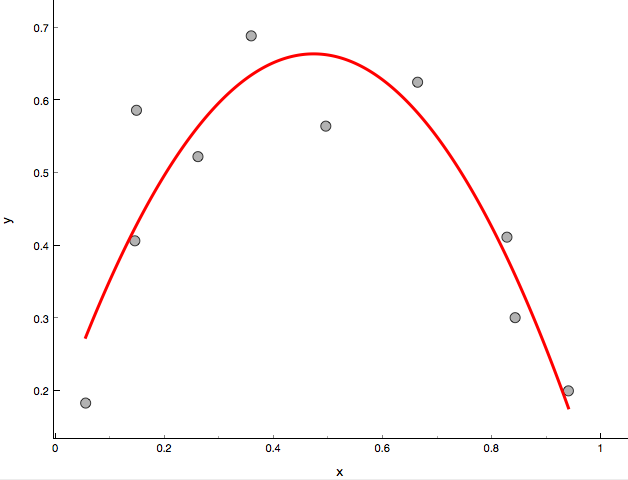
\includegraphics[width=0.45\textwidth]{slike/poly-reg-2.png}\hfill
  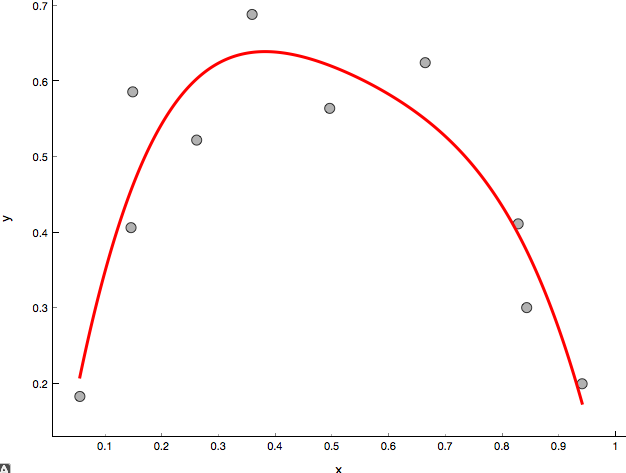
\includegraphics[width=0.45\textwidth]{slike/poly-reg-4.png}
\caption{Polinomska regresija druge in četrte stopnje.}
\label{fig:poly-linear-fit}
\end{center}
\end{figure}

Z dviganjem stopnje polinoma se naš model čedalje bolj prilega učnim podatkom, napovedna napaka oziroma naša kriterijska funkcija pa je čedalje manjša. S polinomsko razširitvijo sedmega reda smo dosegli skoraj popolno prileganje (slika~\ref{fig:poly-linear-fit7}). Vrednost naše kriterijske funkcije gre z dvigovanjem stopnje polinoma proti nič in je dejansko enaka nič takrat, ko je stopnja polinoma oziroma razširitve atributnega prostora enaka $m-1$, kjer je $m$ število primerov.

\begin{figure}[htbp]
\begin{center}
  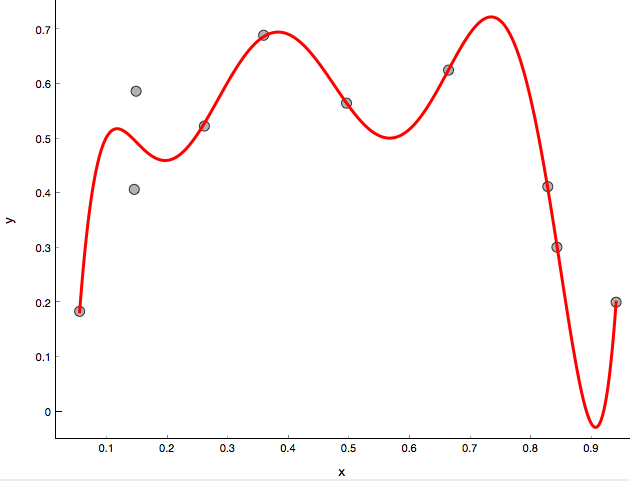
\includegraphics[width=0.45\textwidth]{slike/poly-reg-7.png}
  \hfill
  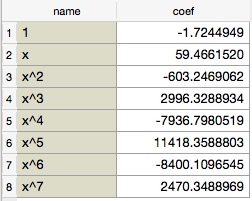
\includegraphics[width=0.45\textwidth]{slike/poly-reg-7-coeff.png}
\caption{Polinomska regresija sedme stopnje in koeficienti modela.}
\label{fig:poly-linear-fit7}
\end{center}
\end{figure}

Navidezno smo problem iskanja modela, ki bi minimiziral kriterijsko fukcijo, z uvedbo polinomske regresije rešili. Pa smo res? Spomnimo se, da je naš cilj gradnje modelov napovedovanje, torej ne samo modeliranje na osnovi učne množice, ampak uporaba modela za napovedovanje primerov, ki jih pri učenju nismo videli in ki so novi. Uporabo polinomske regresije moramo zato preskusiti na tovrstnih primerih, ki jim pravimo tudi testna množica. Pred tem pa se moramo dogovoriti, kako bomo merili uspešnost modela oziroma njegovo napovedno točnost.

\section{Napovedna točnost}

Imejmo testno množico $\cal{T}$ s $k$ primeri, $k=|\cal{T}|$, za katere poznamo njihov atributni opis $x^{(i)}$ in vemo njihov pravi razred $y^{(i)}$. Oceniti želimo napovedno točnost regresijskega modela, ki za $i$-ti primer napove oziroma oceni vrednost njegovega razreda kot $\hat{y}^{(i)}$.

Pri prvi meri za napovedno točnost, ki jo bomo tu uvedli, sledimo dosedanji logiki, da nas predznak napake ne zanima (torej kvadriramo) in da bi radi izračunali povprečno vrednost take, kvadrirane napake. Ker bi želeli, da se napaka izrazi v istih enotah kot vrednosti razreda v učni množici, povprečno kvadrirano napako na koncu še korenimo. Dobimo koren povprečne kvadrirane napake \angl{Root Mean Squared Error}):

$$ {\rm RMSE}(\cal{T})=\sqrt{\sum_{i=1}^k{(y^{(i)}-\hat{y}^{(i)})^2}\over k} $$

Mera RMSE je sicer čisto v redu, a je njena vrednost odvisna od domene odvisne spremenljivke. Na primer, če je ${\rm RMSE}=42.0$ s tem pravzaprav nismo povedali ničesar, saj ne poznamo razpon odvisne spremenljvike. Če smo s tem ocenili težo tovornjakov v tonah, je napaka ogromna, če pa smo njegovo težo ocenjevali v kilogramih, je skoraj zanemarljiva. Bolje bi bilo imeti oceno napake, kjer je ta neodvisna od domene odvisne spremenljivke. Recimo, nekaj, čemur statistiki pravijo delež razložene variance:

$$ R^2({\cal T})=1-{\sum_k (y^{(i)}-\hat{y}^{(i)})^2
  \over \sum_k(y^{(i)}-\bar{y})^2} $$

V imenovalcu ulomka je vsota kvadratov napak, ki bi jo naredili, če bi model napovedoval s povprečno vrednostjo odvisne spremenljivke učne množice. To bi bil prav slab model in pričakujemo, da bo njegova napaka večja, ali pa morda veliko večja od te, ki bi jo naredil boljši model in katerega kvadrat napake izračunamo v števcu ulomka. Za zelo dober model gre člen z ulomkom proti vrednosti 0, ocena $R^2$ pa zato proti vrednosti 1. Slabši modeli pa bodo imeli napako le malo manjšo od napake napovedi s povprečno vrednostjo.

Ocena $R^2$ bo takrat šla proti 0. Delež razložene variance ima zato pričakovano vrednost med 0 in 1. Opozorimo le, da čeprav vemo, da bodo visoke vrednosti $R^2$, torej take blizu 1.0 zaželene, so lahko uporabni tudi modeli z vrednosti $R^2$ blizu nič. Na primer, z modelom, ki ima na testni množici pri napovedi tečaja neke valute $R^2=0.1$ bi obogateli, model z isto točnostjo za napoved jutrišnje povprečne temperature pa bi lahko vrgli v koš.

\section{Ocenjevanje napovedne točnosti}

Naredimo eksperiment: učno množico, ki jo prikazuje slika~\ref{fig:poly-reg-many}, naključno razdelimo na polovico, kjer uporabimo polovico naključno izbranih primerov za učenje linearnega modela, na drugi polovici modela pa testiramo napovedno uspešnost. Za ocenjevanje točnosti smo uporabili $R^2$, in to merili na učni in testni množici.

\begin{figure}[htbp]
\begin{center}
  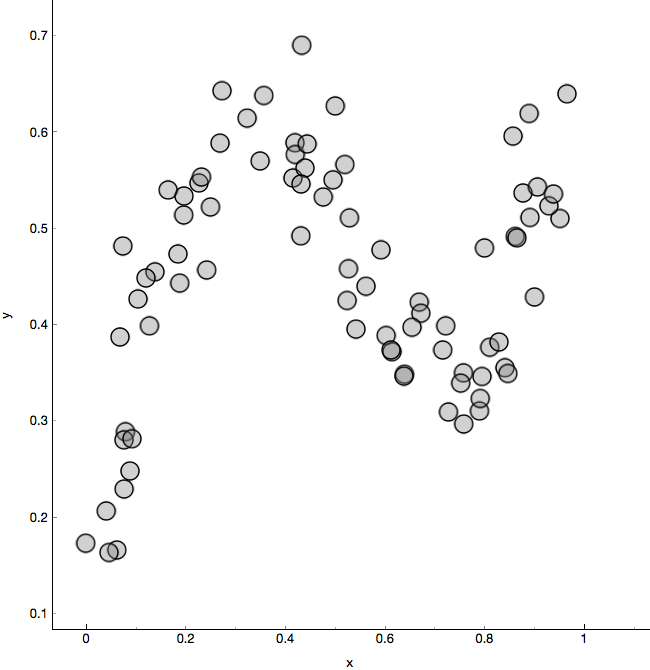
\includegraphics[width=0.45\textwidth]{slike/poly-reg-many.png}
\caption{Množica vseh primerov, ki jih naključno porazdelimo med učno in tesno množico za ocenjevanje gradnjo in ocenjevanje kvalitete modela polinomske regresije.}
\label{fig:poly-reg-many}
\end{center}
\end{figure}

Rezultate kaže tabela~\ref{tab:poly-reg-many-res}. S stopnjo polinomske razširitve atributnega prostora napovedna točnost modela na učni množici monotono narašča. Na množici testnih primerov pa je slika drugačna: s kompleksnostjo modela napovedna točnost nekaj časa narašča, potem pa strmo pade. Pravimo, da se je model preveč prilegel učni množici, postal zato prekompleksen in ni zajel glavnih vzorcev, ki so prisotni tudi v novih primerih.

\begin{table}
  \caption{Delež razložene variance na učni in testni množici (podatki s slike~\ref{fig:poly-reg-many}) za polinomsko regresijo stopnje $k$.}
  \begin{center}
  \begin{tabular}{ccc}
    \hline
    k & učna & testna \\
    \hline
    0 & 0.000 & 0.002 \\
    1 & 0.031 & 0.037 \\
    2 & 0.161 & 0.151 \\
    3 & 0.806 & 0.688 \\
    4 & 0.822 & 0.687 \\
    5 & 0.832 & 0.715 \\
    6 & 0.841 & 0.716 \\
    7 & 0.841 & 0.714 \\
    8 & 0.857 & 0.365 \\
    9 & 0.863 & 0.118 \\
    \hline
  \end{tabular}
  \end{center}
  \label{tab:poly-reg-many-res}
\end{table}

\section{Regularizacija linearne regresije}

Ko višamo stopnjo polinomske razširitve atributnega prostora smo opazili (slika~\ref{fig:poly-linear-fit7}), da parametri modela podivjajo, oziroma postane njihova vrednost zelo visoka. Kar ni nič čudnega, saj se model zelo prilagodi učnim podatkom, funkcija odvisnosti med $x$ in $y$ je zelo razgibana, njeni odvodi pa zelo visoki. Prileganje učni množici se torej izrazi v absolutno velikih vrednostih parametrov modela (absolutno zato, ker so te vrednosti lahko visoke a negativne ali visoke in pozitivne). Želeli bi si manj ``divje'' modele, torej take, kjer bi bili parametri modela po absolutni meri manjši. To željo enostavno izrazimo kot dodatek h kriterijiski funkciji za linearno regresijo:

\begin{equation}
J = {1\over 2m}\sum_{i=1}^m (f(x^{(i)})-y^{(i)})^2 + \eta\sum_{j=1}^n \theta_j^2
\end{equation}

Prvi člen v zgornji enačbi je cenovna funkcija za linearno regresijo, kjer želimo, da se model čimbolj prilega učni množici. Drugi člen pa pravi, da naj bo kvadratna vrednost parametrov takega modela čim manjša. Uporabili smo kvadratno vrednost parametrov, saj nam je vseeno, ali je njihova vrednost pozitivna ali negativna. Pravimo, da smo cenovno funkcijo regularizirali, stopnjo regularizacije pa uravnavamo z vrednostjo $\eta$, katere tipične vrednosti so nizke, recimo 0.1 ali pa 0.01 ali pa celo 0.0001.

Za učenje modela linearne regresije, torej, za določanje vrednosti parametrov $\theta_i$ modela iz podatkov rabimo še izračunati gradient. Izračun je enostaven, saj je enak, kot pri neregularizirani linearni regresiji plus odvod člena za regularizacijo (spodnja enačba velja za $i=1\ldots n$, za $i=0$ pa ostane odvod enak kot prej):

\begin{equation}
{\partial\over\partial\theta_i} J(\theta) = {1\over m}(h_\theta(x)-y)x_i + 2\eta\theta_i
\end{equation}

Ostane le še preskus: ali se, tudi z regularizacijo, lahko preveč prilagodimo manjšemu naboru podatkov v učni množici. Seveda je vse odvisno od stopnje regularizacije $\eta$, a v splošnem (pri primerni vrednosti parametra $\eta$) je odgovor ne. Regularizacija nam pomaga pri preprečevanju prevelikega prileganja. Naj sliki~\ref{fig:poly-reg-compare} je tako primer podatkov in polinomske regresije brez regularizacije in z regularizacijo.

\begin{figure}[htbp]
\begin{center}
  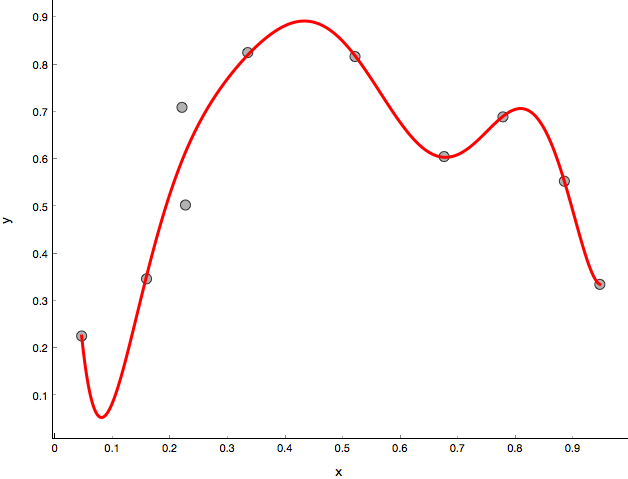
\includegraphics[width=0.45\textwidth]{slike/poly-reg-no.png}
  \hfill
  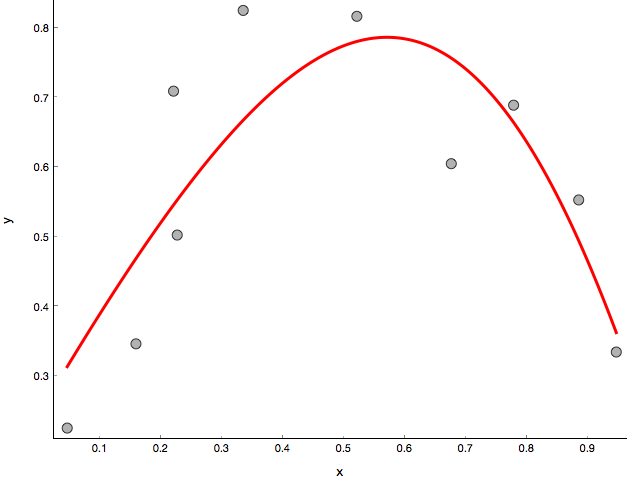
\includegraphics[width=0.45\textwidth]{slike/poly-reg-yes.png}
\caption{Model polinomske regresije stopnje osem brez (levo) in z regularizacijo ($\eta=0.01$, desno).}
\label{fig:poly-reg-compare}
\end{center}
\end{figure}
